%---------------------------------------------------------------------
% TJAA - Example Article - Example.tex
%
% This file format has been adapted from Springer's llncs proc package.
%
% Producer: Springer
% Adapted by Sinan Kaan Yerli, ODTU Fizik Bolumu, Ekim 2010.
%
% Version: 2015-06-15 - 1.1
% Version: 2019-08-01 - 2.0
% Version: 2021-04-01 - 2.1
% Version: 2022-01-01 - 2.2
% 	- added Example-Turkce file using \TRlang
% 	  which explains multi language abstract
% 	- updated explanations in manuscript meta-data notes
% 	- added sections: Astro. Macros, Astro. Journals
% 	- added description for new columntypes
% 	- added section for auth-year commands
% Version: 2022-01-22 - 2.3
%	- added Disclosure section
% Version: 2024-09-01 - 2.4
%	- updated author & address usage with new commands
%	- updated abstract description
%	- updated keyword description
%	- added descr. for new astronomical macros
%---------------------------------------------------------------------
\documentclass[usenatbib]{tjaa}

% 用於Table
\usepackage{array}
\usepackage{tabularx}
\usepackage{booktabs}

\usepackage{amsmath} % 用于数学公式
\usepackage{listings} % 代碼塊宏包
\usepackage{color} % 代碼高亮

\definecolor{dkgreen}{rgb}{0,0.6,0}
\definecolor{gray}{rgb}{0.5,0.5,0.5}
\definecolor{mauve}{rgb}{0.58,0,0.82}

% 设置代码样式
\lstset{ %
    %language=Octave,                % the language of the code
    basicstyle=\footnotesize\ttfamily,           % the size of the fonts that are used for the code
    numbers=none,                   % where to put the line-numbers
    numberstyle=\tiny\color{gray},  % the style that is used for the line-numbers
    stepnumber=2,                   % the step between two line-numbers. If it's 1, each line 
                                    % will be numbered
    numbersep=3pt,                  % how far the line-numbers are from the code
    backgroundcolor=\color{white},      % choose the background color. You must add \usepackage{color}
    showspaces=false,               % show spaces adding particular underscores
    showstringspaces=false,         % underline spaces within strings
    showtabs=false,                 % show tabs within strings adding particular underscores
    frame=single,                   % adds a frame around the code
    rulecolor=\color{black},        % if not set, the frame-color may be changed on line-breaks within not-black text (e.g. commens (green here))
    tabsize=2,                      % sets default tabsize to 2 spaces
    captionpos=b,                   % sets the caption-position to bottom
    breaklines=true,                % sets automatic line breaking
    breakatwhitespace=false,        % sets if automatic breaks should only happen at whitespace
    title=\lstname,                   % show the filename of files included with \lstinputlisting;
                                    % also try caption instead of title
    keywordstyle=\color{blue},          % keyword style
    commentstyle=\color{dkgreen},       % comment style
    stringstyle=\color{mauve},         % string literal style
    escapeinside={\%*}{*},            % if you want to add LaTeX within your code
    morekeywords={*,...}               % if you want to add more keywords to the set
}
%---------------------------------------------------------------------
% Türkçe karakterler ile yazmak ve Türkçe heceleme icin aşağıdaki
% paketin etkin olması zorunludur.
\usepackage[utf8]{inputenc}
%%%%% AUTHORS - PLACE YOUR OWN PACKAGES HERE %%%%%
\usepackage{lipsum}
\newsavebox\verbbox

% 控制圖片位置
\usepackage{float}
%%%%%%%%%%%%%%%%%%%%%%%%%%%%%%%%%%%%%%%%%%%%%%%%%%%%%%%%%%%%%%%%%%%%%%
%%%%                                                              %%%%
%%%% PLEASE DONT DELETE LINES CONTAINING "%%%%TJAA-OZEL"          %%%%
%%%%                                                              %%%%
%%%% PLEASE DONT CLEAR -OR- MOVE OUT OF THE LINE THE TEXTS        %%%%
%%%%   CONTAINING "%%%%TJAA-OZEL"                                 %%%%
%%%%                                                              %%%%
%%%% IF YOU HAVE YOUR OWN TEX FILE, IN THE SAME WAY USED IN       %%%%
%%%% THIS FILE POPULATE CORRESPONDING LINES OR LINE ENDINGS       %%%%
%%%% WITH "%%%%TJAA-OZEL" **MANUALLY**.                           %%%%
%%%%                                                              %%%%
%%%% ------------------------------------------------------------ %%%%
%%%% LUTFEN "%%%%TJAA-OZEL" SATIRLARINI SILMEYIN                  %%%%
%%%%                                                              %%%%
%%%% LUTFEN SATIR SONLARINDAKI "%%%%TJAA-OZEL" BOLUMLERINI        %%%%
%%%%   SILMEYIN YA DA SATIRDAN KOPARMAYIN                         %%%%
%%%%                                                              %%%%
%%%% ONCEDEN KODLANMIS BIR TEX DOSYANIZ VARSA BU DOSYADA          %%%%
%%%% KULLANILDIGI GIBI "%%%%TJAA-OZEL" SATIRLARINI VE SATIR SONU  %%%%
%%%% EKLENTILERINI **ELLE** EKLEYIN                               %%%%
%%%%                                                              %%%%
%%%%%%%%%%%%%%%%%%%%%%%%%%%%%%%%%%%%%%%%%%%%%%%%%%%%%%%%%%%%%%%%%%%%%%

%%%%TJAA-OZEL:BASLIK%
% NOTES (title):
% 1) If you need to put a \newline in the title
%    then you HAVE TO specify the short title
%    DONT USE [] (short title) if your title not overlapping short author
\title[Enhancing Detection of Anomalies on IIoT Networks]{ENHANCING DETECTION OF ANOMALIES ON IIOT NETWORKS WITH FINE-TUNED LARGE LANGUAGE MODELS}%%%%TJAA-OZEL:TITLE%

% NOTES (authors):
% 1) For single author don't number single affiliation addreess.
% 2) If you need two or more lines of authors, use \newauthor (see below usage)
% 3) ORCID is required for ALL authors
% 4) Short author should be either A.U. Thor et.al -or- A. U. Thor
% 5) Depending on the language \others will be either "et al." or "v.ark."
\author[H. Author \others]{%
Huang Po-Hsun\thanks{fh831.cp9gw@gmail.com}
% \\
% NOTES (List of institutions):
% 1) Don't put \\ at the last institution
% \adrid{1}University, Department, City Post Code, Country
}%%%%TJAA-OZEL:AUTHOR%
% These dates and numbers will be filled out by the publisher
\date{October 29, 2024}
%
\renewcommand{\pubyear}{2024}
\renewcommand{\volume}{0}
\renewcommand{\issue}{0}


\begin{document}
% Don't change these 3 lines
\label{firstpage}
\pagerange{\pageref{firstpage}--\pageref{lastpage}}
\maketitle{M00-0000}

\begin{abstract}
This research plan proposes to enhance the detection of anomalies in Industrial Internet of Things (IIoT) networks
by fine-tuning Large Language Models (LLMs). As the complexity and interconnectivity of IIoT networks increase,
anomaly detection has become a critical challenge, especially in terms of potential security threats
and operational failures. The plan explores the use of machine learning and deep learning algorithms to analyze
the vast amounts of data generated by IoT devices, enabling real-time anomaly detection. The focus of the research
is on combining traditional statistical methods with modern machine learning approaches to enhance detection capabilities
and reduce false positives. Additionally, the study investigates how fine-tuning LLMs can improve their performance in
specific tasks or domains, including the use of Reinforcement Learning with Human Feedback (RLHF) methods and Low-Rank
Adaptation (LoRA) techniques to optimize model outputs and reduce computational overhead. The goal of this research
is to build an adaptable anomaly detection model suitable for a variety of IIoT scenarios and devices,
thereby enhancing the resilience and security of interconnected industrial systems. By leveraging the time series
learning capabilities of large models to understand multiple patterns, distinguishing between normal fluctuations and abnormal situations,
and reducing false alarm rates, we aim to achieve a 5-10\% increase in accuracy through fine-tuning LLMs and enable
the model to adapt more quickly to new or complex anomalies.
\end{abstract}

\begin{keywords}
% W A R N I N G : ***** N O  T U R K I S H  K E Y W O R D S *****
IIoT Device Control, IIoT Networks, Large Language Models, Intelligent Agents
% W A R N I N G : ***** N O  T U R K I S H  K E Y W O R D S *****
\end{keywords}



% 建議的區分

%     引言:主要集中於為何研究這個主題,問題的概述。
%     文獻綜述:分析和評價現有研究,指出具體的研究空白。
%     研究目的與問題:清楚界定你的研究將針對哪些具體問題,並且可能提到這些問題的挑戰。

% 這樣可以避免重複,同時讓每個章節各自突出其重點。你可以在引言中簡單提及問題,然後在文獻綜述中深入分析,
% 最後在研究目的與問題中明確你自己的研究方向。
%%%%TJAA-OZEL:BILDIRI%
% - - - - - - - - - - - - - - - - - - - - - - - - - - - - - - - - - - -
% 1. 引言 (Introduction)

%     研究的意義和價值:強調研究的重要性,說明為何這個主題值得研究。
%     問題陳述:清晰地描述你要解決的具體問題,但不需要過於詳細,主要是引入讀者。
\section{Introduction}
IIoT technology and AI have
emerged as two of the most transformative technologies of our
time \citep{zuo2024federated}.
On the other hand,
LLMs can understand and generate
human-like text, based on extensive training on diverse datasets
with billions of parameters \citep{kalita2024large}.
Task-oriented communications are an important
element in future intelligent IIoT systems. Existing IoT systems,
however, are limited in their capacity to handle complex tasks,
particularly in their interactions with humans to accomplish these
tasks \citep{cui2024llmind}. 
The industry need to be good at making use of the LLM,
which has been popular in recent years, to improve
the shortcomings of the IoT in device networks.

The detection of anomalies in IIoT networks is particularly significant
due to the potential consequences of undetected issues,
such as production downtime, safety hazards, or data breaches.
Recent studies have highlighted the effectiveness of combining
traditional statistical methods with modern machine learning approaches
to enhance detection capabilities \citep{9034736}.
For instance, techniques like unsupervised learning and reinforcement
learning have been applied to improve the accuracy of anomaly
detection systems while minimizing false positives.
Additionally, researchers have emphasized the importance of
feature extraction and selection, as well as the integration of
domain knowledge, to better identify relevant patterns in the data.

Overall, the landscape of anomaly detection in IIoT networks is evolving,
with ongoing research aimed at developing more robust and adaptive
systems. By addressing the unique challenges posed by IIoT environments,
these efforts aim to enhance the resilience and security of
interconnected industrial systems.

LLMs have made significant strides
in the field of natural language processing in recent years.
These models are pretrained on vast amounts of text data,
enabling them to generate fluent text and understand complex
language patterns. As interest in LLMs has grown,
researchers have begun exploring how to effectively fine-tune
these models to better adapt to specific tasks or domains.
The fine-tuning process typically involves further training the model
on specialized datasets, allowing it to perform better in specific
applications. For example, using supervised learning methods can
help the model learn more precise task-related features\citep{chen2020big}.

Recent studies have shown that fine-tuning large models
can not only enhance their performance on specific tasks
but also improve their understanding and generative capabilities
in context\citep{ding2023parameter}.
Some researchers have proposed combining reinforcement
learning with human feedback (RLHF) methods to enhance
the quality of model outputs, especially in generative
tasks\citep{wu2023fine}.
Additionally, emerging techniques like Low-Rank Adaptation (LoRA)
have been introduced to reduce the computational overhead
and resource requirements during the fine-tuning process.
These research efforts are gradually enriching the application
potential of LLMs, showing positive results across various domains,
from chatbots to text summarization.

% \subsection{Objectives}
As IIoT networks become more complex and interconnected, the detection of anomalies
has emerged as a critical challenge, with researchers exploring
various techniques to identify unusual patterns in network traffic
that may indicate potential security threats or operational failures\citep{Reuer_2022}.
These techniques often leverage machine learning and deep learning algorithms
to analyze the vast amounts of data generated by IoT devices,
enabling real-time detection of anomalies\citep{alharbi2022novel}.

The continuous flow of data collected by IoT devices, has revolutionised
our ability to understand and interact with the world across various applications\citep{shirali2024llm}.
In \citet{cui2024llmind}, they Design an LLM-based taskoriented AI agent framework that enables effective collaboration
among IoT devices in Figure~\ref{fig:llmFramwork}\citep{cui2024llmind}.
However, although their system designed the conversion between natural
language and code and executed it on IIoT devices,
they did not further consider the problem of network anomalies in IIoT devices.
This system is highly dependent on transmission between networks.
If a network failure occurs, there is no response to troubleshoot the problem.

Additionally, LLMs have provided highly effective methodologies and solutions
in various cybersecurity sectors \citep{mohamed2024efficient}.
As the frequency and diversity of cybersecurity attacks continue to rise, the
importance of incident detection has significantly increased \citep{thandi2024revolutionizing}.
Our goal is to more accurately detect abnormal patterns through the time series learning capabilities
of deep models. Use large models to understand multiple patterns to distinguish normal fluctuations from
abnormal situations and reduce false alarm rates.
Finally, an adaptable anomaly detection model is built that is suitable for a variety of IIoT scenarios and devices.

\begin{figure}
  % \vspace{10 cm}
  \centering
  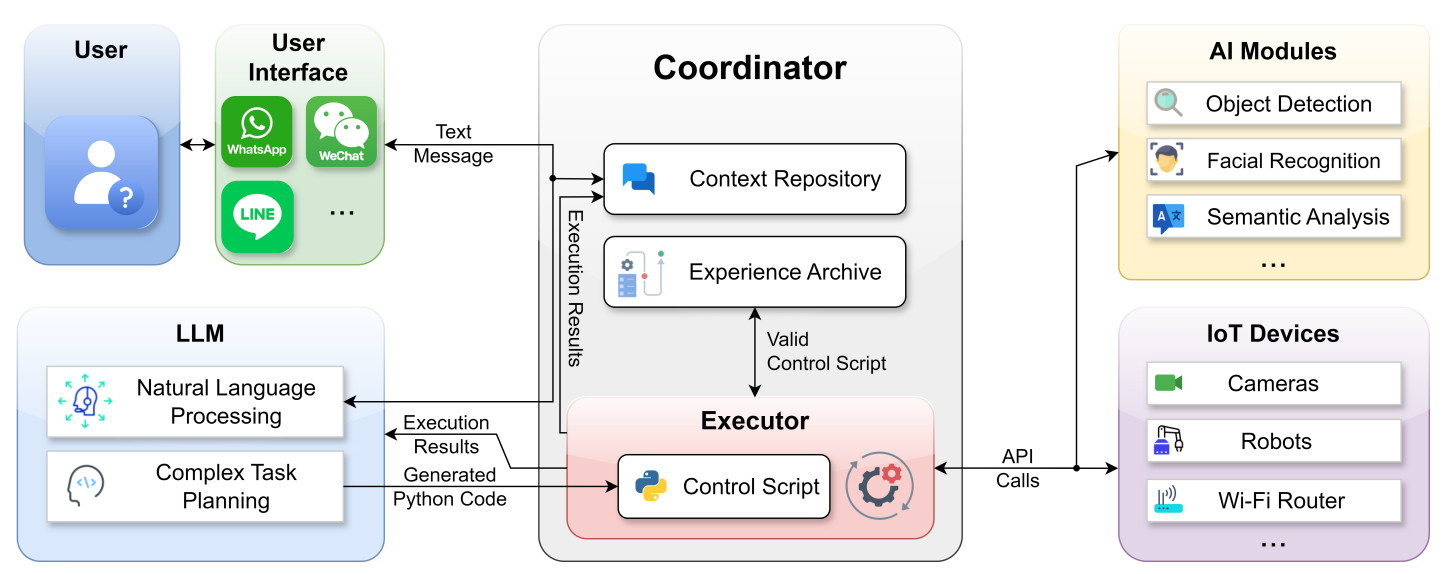
\includegraphics[width=0.5\textwidth]{./img/system_diagram.png} % 这里替换为图像文件名
  \caption{System diagram}
  \label{fig:llmFramwork}
\end{figure}

% \section{Expected Outcomes}
We anticipate establishing a new IIoT framework that enhances resilience against
potential threats and anomalies in existing IIoT network security.
This framework aims to improve the effectiveness of industrial IIoT
security through validated evidence, contributing to the knowledge
base of this emerging field.

With fine-tuned LLMs demonstrating their versatility beyond
natural language tasks in industrial contexts, we expect the model
to achieve higher accuracy and recall rates after fine-tuning,
with an anticipated increase of 5-10\% in accuracy.
The model will adapt more swiftly to new or complex anomalies,
thereby expanding its capability to detect various types of
attacks or anomalies.

Finally, we will maintain the model’s adaptability to
emerging IIoT anomalies through regular fine-tuning or
the incorporation of new data.
% \newpage
% - - - - - - - - - - - - - - - - - - - - - - - - - - - - - - - - - - -
% 2. 文獻綜述 (Literature Review)

%     相關研究回顧:集中在已有文獻的分析上,介紹前人的研究成果、方法、結論和不足之處。
%     研究空白:指出現有文獻中的不足,這部分可以進一步細化,解釋為什麼這些不足需要你的研究來填補。
% \section{Literature Review}
% - - - - - - - - - - - - - - - - - - - - - - - - - - - - - - - - - - -
% 3. 研究目的與研究問題 (Objectives and Research Questions)

% 研究目的:具體闡述你的研究目標,明確你的研究將要達到的結果。
% 具體問題和假設:在這裡詳細列出你要解決的具體研究問題或假設,並簡要提及這些問題的挑戰。
\section{Research Questions and Hypotheses}


% \subsection{Research Questions}
Below are posed to optimize network detection based on their designed IIoT task-oriented framework,
which may help identify potential challenges, define research directions,
and evaluate the actual performance of the model.

\subsection{Fine-tuning Model}
% Model Adaptability
Firstly, Can a large model, once fine-tuned, adapt to different IIoT devices?
In which device environments does it perform best?
I think that fine-tuning a large model significantly improves
the accuracy and recall rates of IIoT network anomaly detection,
making it better suited for complex anomaly patterns than traditional detection methods.

% Model Scalability
On the other hand, the model flexibly adapt to emerging IIoT anomaly patterns,
or does it require periodic fine-tuning or retraining?
We can hypothesize that multi-task fine-tuning (e.g., anomaly detection and classification in parallel)
can further improve the model’s ability to identify specific types of anomalies.

\subsection{Data Processing}
% Data Requirements
Some questions that arise when we collect IIoT data is:
Does fine-tuning an IIoT anomaly detection model require a large amount of data?
How do data scale and quality impact detection effectiveness?
A moderate amount of IIoT anomaly data can greatly improve the model's generalization ability,
enabling it to maintain high detection accuracy across various IIoT environments.

% Knowledge Base \& RAG Vector Database
In Figure~\ref{fig:fsmProcedure}, if the RAG vector library and knowledge base are added,
can the command problems of the system be better located?
establishing this node requires additional resources.
Because in the industrial Internet of Things,
the environment that isolates the external network needs to be considered,
it is necessary to establish its own LLM independently.
Compared with the resources consumed by running LLM,
a vector library can be added to speed up the troubleshooting process.

\begin{figure*} % [h] 表示将图像放置在此处
  % \centering
  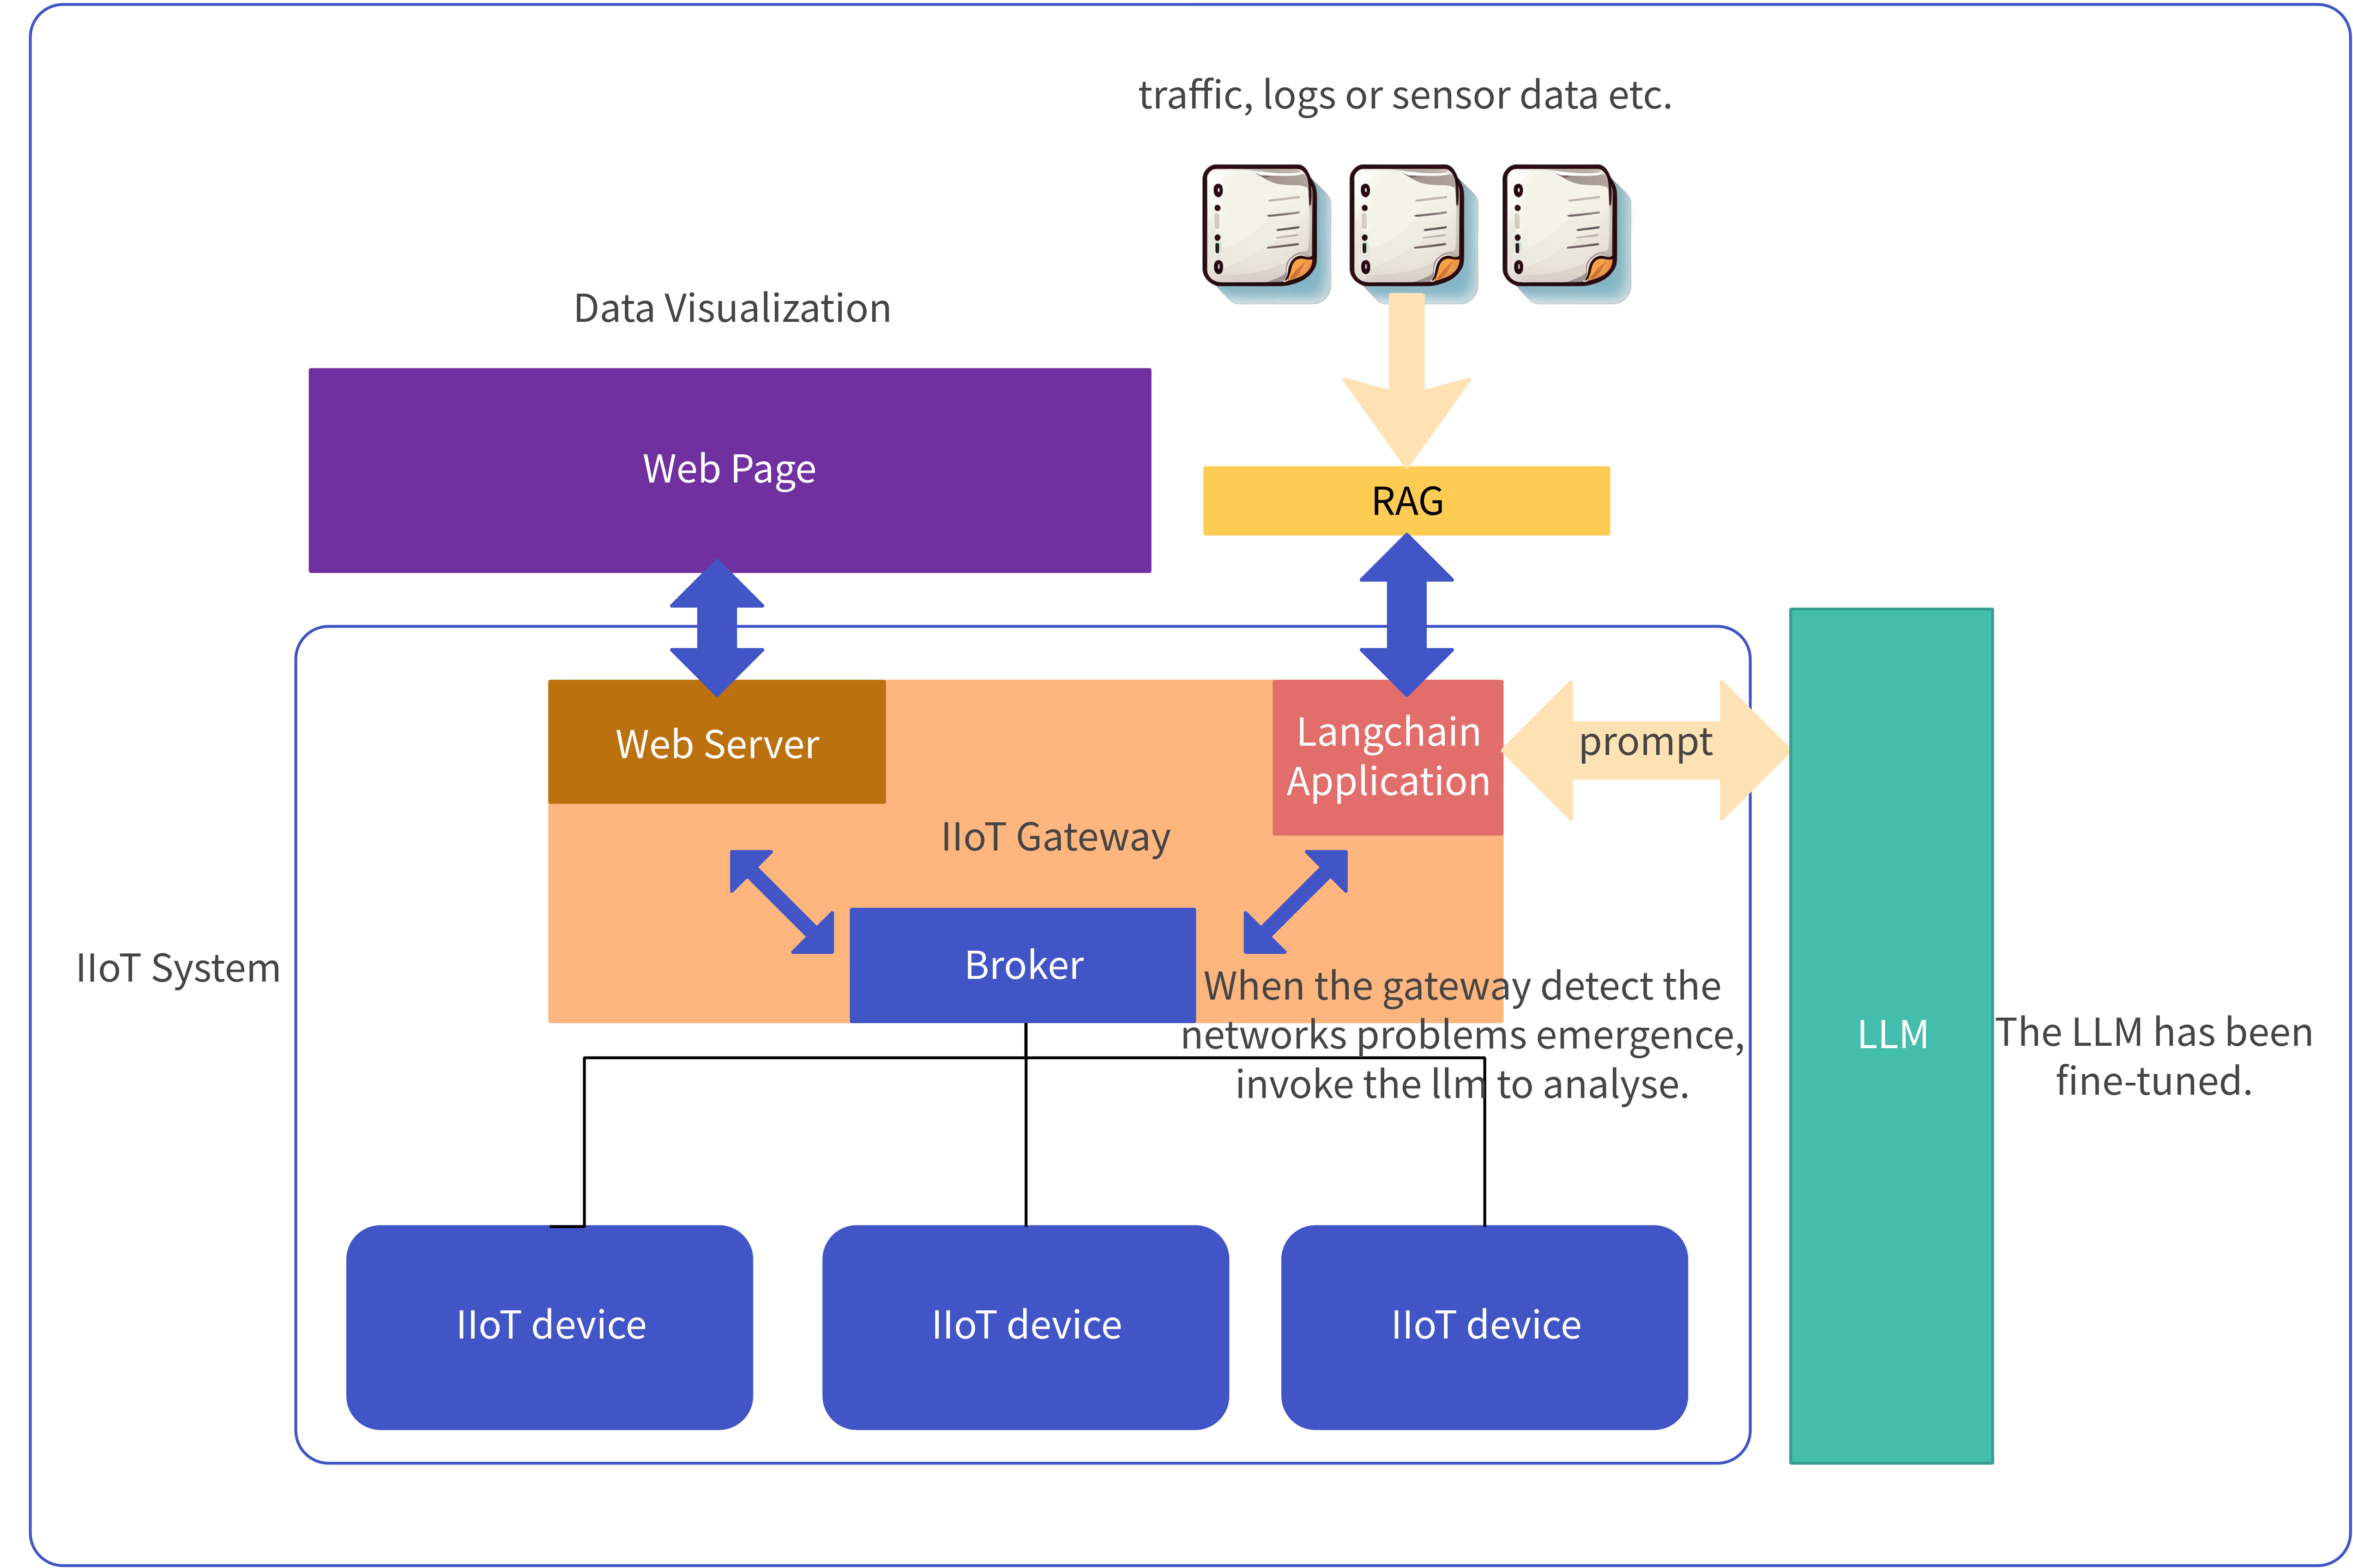
\includegraphics[width=0.6\textwidth]{./img/my_iiot_system.jpg} % 这里替换为图像文件名
  \caption{The IIoT System designed by me}
  \label{fig:fsmProcedure}
\end{figure*}

% Data Privacy
However, Data privacy is a serious and unavoidable issue.
How can IIoT data privacy be effectively protected
during data collection and model deployment?
The fine-tuned model is suitable for real-time anomaly detection,
with a response time of 1-2 seconds for most IIoT network anomalies.

\subsection{Performance and Cost}
% Real-time Detection
About Performance, can the fine-tuned model meet real-time detection requirements
in practical applications? If there is latency,
how can it be optimized?
I assume that the false positive rate of a fine-tuned large model will be
substantially lower than traditional statistical or rule-based methods,
thereby reducing interference in anomaly detection.

% False Positive and False Negative Rates
Then, we need to seriously think about the cost issue.
What are the computational, storage, and energy costs when deploying
the fine-tuned model in IIoT environments?
Can it effectively operate on resource-limited devices?
Distributed fine-tuning can effectively reduce the computational
burden on IIoT devices without significantly impacting
detection performance.

% Resource Consumption
What are the computational, storage, and energy costs when
deploying the fine-tuned model in IIoT environments?
Can it effectively operate on resource-limited devices?
The model’s accuracy in detecting new types of anomalies will degrade over time,
but incremental fine-tuning can restore performance.

% - - - - - - - - - - - - - - - - - - - - - - - - - - - - - - - - - - -
% 4. 研究方法 (Methodology)

%     研究設計:說明研究的整體設計,定性或定量研究,或混合方法。
%     數據收集與分析:具體說明數據的收集方法(例如問卷、訪談、實驗等)和分析方法。
\section{Methodology}
The research will follow a systematic approach to develop and evaluate
the proposed anomaly detection framework.
The methodology includes the following steps.

\subsection{Technical Selection}

Models suitable for handling time series, such as T5, GPT,
or transformer-based time series models,
can be selected and fine-tuned for IoT data.
As shown in Table~\ref{tab:comparison}, Fine-tune the model using labeled normal/abnormal
IoT network data to enable the model to recognize common anomaly patterns.

\begin{table*}
  \centering
  \caption{Comparison of Different Methods}
  \label{tab:comparison}
  \begin{tabularx}{\textwidth}{>{\raggedright\arraybackslash}p{2.5cm} X X X}
      \toprule
      \textbf{Feature} & \textbf{LoRA} & \textbf{RLHF} & \textbf{MoE} \\
      \midrule
      \textbf{Method Type} & Parameter-efficient fine-tuning. & Training optimization. & Model architecture. \\
      \textbf{Core Goal} & Efficiently fine-tune the model. & Enhance the quality of generated content through human feedback. & Improve model performance through selective activation. \\
      \textbf{Suitable Scenarios} & High task adaptability, minimal parameter adjustments needed. & User interaction, dialogue systems. & Multi-task learning, handling complex inputs. \\
      \textbf{Advantages} & Resource-saving, lightweight fine-tuning. & Aligns with human preferences, high-quality output. & Large parameter count but controlled computational load. \\
      \textbf{Implementation} & Low-rank matrix insertion. & Reward model + reinforcement learning. & Mixture of experts network + sparse activation. \\
      \textbf{Cost} & Relatively low. & Relatively high. & High. (but less computation during inference) \\
      \textbf{Complexity} & Low. & High.(involves human feedback and reinforcement learning) & High.(requires expert selection and sparse activation) \\
      \bottomrule
  \end{tabularx}
\end{table*}

% RLHF
Further fine-tune the model using expert feedback after initial fine-tuning to optimize sensitivity to anomaly detection.
The reward model for RLHF has proven effective in fine-tuning Large Language Models
(LLMs)\citep{zhang2024prototypical}.

RLHF optimizes model outputs through human feedback.
The training process typically consists of two steps:
first, training the model using supervised learning,
and then fine-tuning the model using reinforcement
learning based on human feedback. % 去掉 arvix
Formula\ref{eq:RLHF_equation}:
\begin{equation}
  Q(s, a) \gets Q(s, a) + \alpha \left( r + \gamma \max_{a'} Q(s', a') - Q(s, a) \right)
  \label{eq:RLHF_equation} % 为公式添加标签以便引用
\end{equation}

% LoRA
SLoRA(2024) observe that this paradigm presents significant opportunities
for batched inference during serving\citep{sheng2024slora}.
So, we use LoRA for lightweight fine-tuning to save resources.

SLoRA introduces low-rank matrices for fine-tuning the model,
thereby reducing the number of parameters that need to be trained.
The core idea is to decompose the weight matrix $W$ into two low-rank
matrices $A$ and $B$, updating only these two matrices.% arxiv
Its equation is \ref{eq:LoRA_equation}.

\begin{equation}
  W' = W + A \cdot B
  \label{eq:LoRA_equation} % 为公式添加标签以便引用
\end{equation}

% MoE
MoE combines different experts (i.e., sub-models or networks)
with the aim of activating only a subset of these "experts" based
on the specific needs of the input task.
LLM-HAS innovative framework leverages a Mixture
of Experts (MoE) approach, augmented with LLMs, to analyze
users’ personalized preferences and potential health risks from
additional textual job descriptions\citep{gao2024guiding}.

MoE combines multiple expert models, dynamically selecting which experts
to activate to improve model efficiency. By activating only a subset of
experts during inference, it conserves computational resources. %arxiv
Formula\ref{eq:MoE_equation}:
The expression $y$ is equal to the sum of the products of $g_i$ and $E_i(x)$ for all $i$ belonging to the set $S$.

\begin{equation}
  y = \sum_{i \in S} g_i \cdot E_i(x)
  \label{eq:MoE_equation} % 为公式添加标签以便引用
\end{equation}

Where $S$ is the set of activated experts and $g_i$ represents the gating output.
Below is the algorithm for MoE.

Furthermore, the Hugging Face Transformers library and Datasets API can be utilized for
managing datasets and model fine-tuning tasks,
while DeepSpeed can be employed for distributed training and deployment.
It serves as a versatile framework that offers flexible fine-tuning tools.
However, techniques such as LoRA, RLHF, and MoE are more targeted approaches
designed for specific fine-tuning needs and scenarios.
Therefore, I don't choose the Transformers library as the tool for fine-tuning
large models in this context.

\subsection{Data Preparation}

Gather traffic, logs, and sensor data from IoT devices over a period.
Focus on collecting and labeling anomalies and normal events occurring
in actual network environments.

Then, extract features (e.g., traffic peaks, connection frequencies, packet sizes)
from the data and remove noise. Data augmentation techniques can be
used to expand anomaly samples.

Finally, organize data into time series input formats,
such as sliding window sequences, for the model to learn
inter-event relationships.

\subsection{Fine-Tuning Model}

We will select an appropriate LLM and fine-tune it on the collected IIoT data. As mentioned in the work of
\citet{sarabi2023llm}.First fine-tune the model using general network data to learn basic network patterns,
then use IoT-specific data for further fine-tuning to learn specific patterns.

Implement multi-task learning to enable the model to perform anomaly detection while also
classifying types of anomalies (e.g., identifying DDoS attacks, packet loss).

\subsection{Evaluation and Validation}

The fine-tuned LLM will be trained on the IIoT dataset, and its performance will be
validated using a separate validation set to ensure the model's effectiveness in detecting anomalies.
Compare with traditional detection models (e.g., rule-based or statistical analysis methods) to analyze
the advantages and shortcomings of the fine-tuned large model.

The performance of the fine-tuned LLM will be compared with traditional anomaly detection methods to
evaluate its improvement in accuracy and efficiency.
The model will be deployed in a real-world IIoT network setting to test its practical
applicability and robustness in various operational scenarios.
% - - - - - - - - - - - - - - - - - - - - - - - - - - - - - - - - - - -
% 5. 預期結果 (Expected Outcomes)

%     結果描述:預期的研究結果及其對學術界或實踐界的貢獻。
% - - - - - - - - - - - - - - - - - - - - - - - - - - - - - - - - - - -
\section{Conclusion}
In this research plan, I analyze the current state of research on the integration
of IIoT and LLMs in the fields of monitoring and control.
Recent studies on IIoT device control have utilized OpenAI
to generate control code for these devices.

I propose a framework for fine-tuning large models to
enhance the detection of network anomalies in IoT devices
that integrate LLM control systems. Frameworks such as LoRA,
RLHF, and MoE, which are tailored for specific scenarios,
can effectively address troubleshooting in network anomaly
situations, thereby reducing time costs and improving efficiency.

Additionally, it is essential to consider data collection and
significant cost factors. Ultimately, the goal is to achieve a
5-10\% increase in efficiency, improving the control framework
for industrial IoT research.


% Reference
\bibliographystyle{tjaa}
\bibliography{Example}

\label{lastpage}
\end{document}
